\begin{enumerate}
  \item Go to: menu ($\equiv$) $\gg$ Options/Preferences $\gg$ Advanced
  $\gg$ Certificates $\gg$ View Certificates $\gg$ Your Certificates.\\[1em]%
  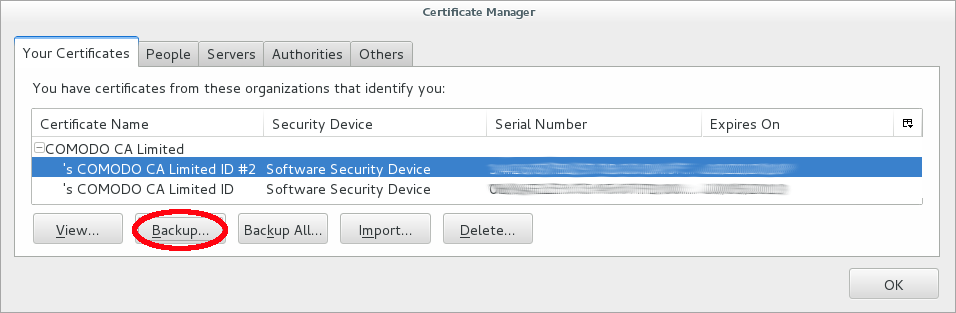
\includegraphics[width=0.7\textwidth]{images/firefox_cert_settings.png}
\item Highlight the line showing your new key.  It will be under the
  name of the CA you chose (e.g. the line under ``COMODO CA Limited''
  if you chose Comodo).
\item %\raisebox{0.6\baselineskip}{\parbox[t]{0.9\textwidth}{%
      %\begin{wrapfigure}{r}{0.7\textwidth}%
      %  \includegraphics[width=0.7\textwidth]{mailapp_firefox_cert_settings.png}
      %\end{wrapfigure}
  Click ``\texttt{Backup...}'' to export the key.
\item Save the file somewhere with a filename of your choice.  It will
  likely be given a \verb|.p12| extension.
\item\label{makebupw} You will be prompted for a password for the
  backup file.  A weak password is fine, because this backup file will
  not be transmitted or retained for long.  You will import it into
  Outlook locally, and then you will delete the backup file.
\end{enumerate}
